\section{Fabrication and characterization}\label{sec:fabrication}

The appealing theoretical predictions together with potential applications in logic, memory and sensor devices~\cite{Allwood02,Allwood05,Parkin08,Parkin15} determine the recent rapid development of fabrication methods for the needs of curvilinear magnetism. As it was shown in Sec.~\ref{sec:theory_1D} and Sec.~\ref{sec:curvature_effects}, the resulting magnetic responses of flat curvilinear wires are mainly predetermined by the choice of geometry and its lateral sizes. Thus, to form a curved structure for the experimental investigation of the curvature-induced effects it is necessary to preserve an immutability of the structure's cross-section along a fabricated geometry. Therefore, it is required a lateral expansion of the wire along the unit vectors of the Frenet-Serret basis according to the Eq.~\eqref{eq:Stripe_param} and Fig.~\ref{fig:TNB}. This allows to obtain a flat three-dimensional stripe with homogeneous geometrical properties: the curvature distribution is preserved as for a curvilinear wire and cross-section along the stripe length remains unchanged. To fabricate flat curvilinear systems it is important to rely on methods that provide predetermined material and geometrical properties of curvilinear structures during the fabrication. 

%\subsection{Geometrical construction}
%
%To form a curved structure for the experimental investigation of the curvature-induced effects it is necessary to preserve an immutability of the structure's cross-section along a fabricated geometry. Therefore, it is required a lateral expansion of the wire along the unit vectors of the Frenet-Serret basis (Fig.~\ref{fig:Parabola_stripe_geometry}(a)), which allows to obtain a flat three-dimensional stripe with homogeneous geometrical properties: the curvature distribution is preserved as for a curvilinear
%wire and cross-section along the stripe length is unchanged. The resulting shape is parametrized as follows
%\begin{equation} \label{eq:Stripe_param}
%\vec{r}(s,w,h) = \vec{\gamma}(s) + w \, \vec{e}_\textrm{N}(s) + h \, \vec{e}_\textrm{B}(s),
%\end{equation}
%where $w$ and $h$ being width $w \in [-W/2,W/2]$ and thickness $h \in [-H/2,H/2]$ of the stripe, respectively, see Fig.~\ref{fig:Parabola_stripe_geometry}(c) and (d). When the stripe is constructed in this way, the shape parameters remain unchanged within the Frenet-Serret basis up to the critical curvature $\kappa^\textrm{c}_0 = 2/W$. For $\kappa_0>\kappa^\textrm{c}_0$, there appears widening in the central part of the stripe due to the overlap of parabolic branches, Fig.~\ref{fig:Parabola_stripe_geometry}(b).
%
%\begin{figure*}
%	\begin{center}
%		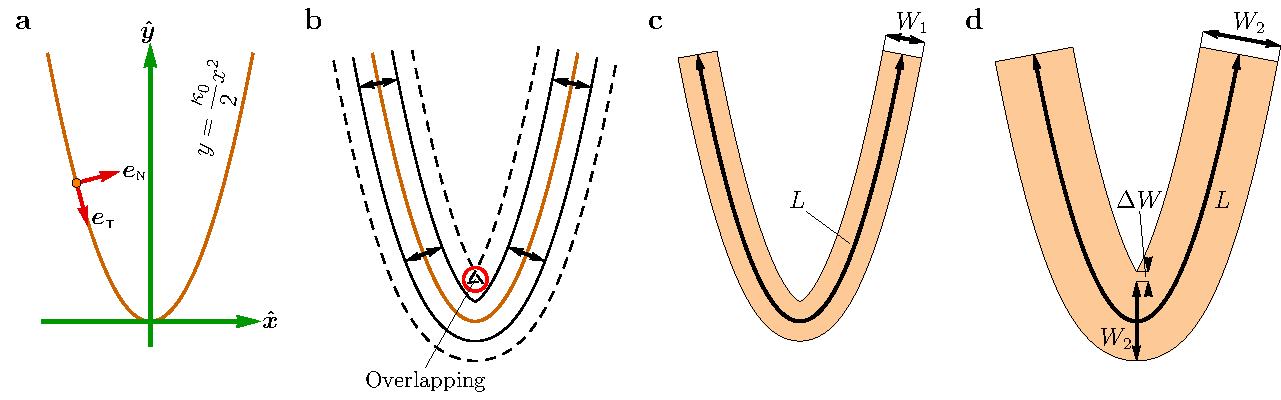
\includegraphics[width=0.9\linewidth]{fig_stripe_construction.pdf}
%	\end{center}
%	\caption{\textit{Geometrical construction of a parabolic stripe.}~(a), One-dimensional parabolic wire in a Cartesian frame of reference.~(b), Schematic picture of a parabolic stripe geometry construction from one-dimensional wire expansion along the normal direction $\vec{e}_\textrm{N}$.~(c) and (d), Show the resulting stripe geometries with two different widths $W_1$ and $W_2=2 W_1$, respectively. Local widening in the apex area of the parabolic stripe is indicated by $\Delta W$.}
%	\label{fig:Parabola_stripe_geometry}
%\end{figure*}	

%==================================================================\
\begin{figure}[t]
	\centering
	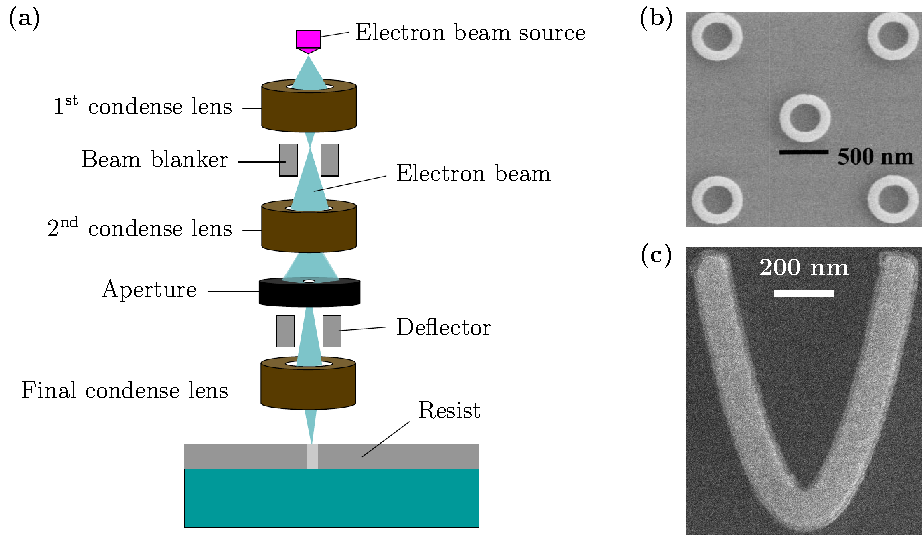
\includegraphics[width=0.85\textwidth]{fig_EBL}
	\caption{\label{fig:EBL_schematics}%
		\textbf{Electron beam lithography and flat curvilinear magnetic structures.} \textbf{(a)}, Schematic illustration of electron beam lithography. Adapted with permission from~\cite{Pimpin12}. \textbf{(b)} and  \textbf{(c)}, Scanning electron images of Co rings with diameter of 520~nm and Py nanostripe with 2~$\mu$m length, respectively. Adapted with permission from \cite{Castano03} and \cite{Volkov19c}.  
	}
\end{figure}
%==================================================================/


\subsection{Lithographic methods}

Standard lithographic techniques combined with thin film deposition represent the first group of methods, that allow to fabricate two-dimensional curved magnetic objects. One of the most developed techniques among this group is Electron Beam Lithography (EBL) method, which allows to ensure shape retention of the patterned geometry and achieve high spatial resolution down to dozens of nanometers. A typical EBL system contains a precise emission source of electrons and necessary optics for the control and focusing of electron beam, see Fig.~\ref{fig:EBL_schematics}. The predetermined shape of the object is drawn in a electron-sensitive resist, whose solubility is changing under the electron beam exposure. This enables it selective removal of either the exposed (positive resist), or non-exposed (negative resist) regions of the resist by immersing it in a chemical developer. The remaining parts of the resist are using either for filling the remaining spaces between them with required material composition, or as a protection of the initially deposited layers from ion-beam etching. The resulting nanostructure could be revealed by removing the remaining resist in a specific solvent. This approach provided the opportunity to study magnetic processes in curved nanostripes~\cite{Lewis09,Nahrwold09,Glathe12} and nanorings~\cite{Castano03,Klaui03a,Klaui05a,Klaui08,Richter16,Mawass17} (see Fig.~\ref{fig:EBL_schematics}(b)) to address DW dynamics and automotion~\cite{Mawass17} for prospective memory~\cite{Hayashi07,Parkin08,Parkin15} and logic~\cite{Allwood02,Allwood04,Allwood05,Hrkac11} devices, parabolic nanostripes (see Fig.~\ref{fig:EBL_schematics}(c)), as well as the concept of magnon-based processing of binary data~\cite{Schneider08,Lee08e,Vogt12,Vogt14,Chumak15}.



\subsection{Ion-induced methods}

%==================================================================\
\begin{figure}[t]
	\centering
	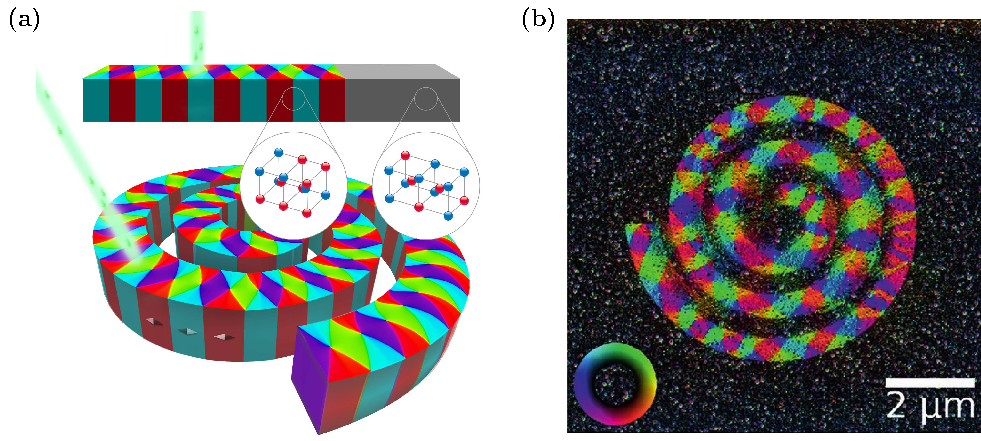
\includegraphics[width=0.9\textwidth]{fig_FIB_method}
	\caption{\label{fig:FIB_schematics}%
		\textbf{Focused Ion Beam method for direct writing of magnetic patterns.} \textbf{(a)}, Schematic illustration of the stylus-like writing of magnetic patterns with different shapes. \textbf{(b)}, Periodic domain wall pattern obtained in a spiral structure by means of scanning transmission electron microscopy.
	}
\end{figure}
%==================================================================/

Another perspective method for the fabrication of flat curved magnetic objects relies on activation of nonmagnetic films through the introduction of chemical disorder. This phenomenon is based on the ion-induced manipulation of the electronic band structure and increasing number of nearest-neighbor magnetic sites inside the initially nonmagnetic films. For instance, Fe$_60$Al$_40$ alloy is paramagnetic in a chemically ordered cubic B2 phase (space group221), while in the disordered body-centered cubic A2 phase (space group 229) it becomes ferromagnetic~\cite{Fassbender08,Bali14}. The B2-A2 phase transition could be introduced by means of energetic ions, whose impact on Fe and Al atoms cause random arrangement in the film. The utilization of the Focused Ion Beam (FIB) in terms of Helium Ion Microscope (HIM) allows to achieve well-defined shapes of magnetic structures with sub-50~nm resolution~\cite{Bali14}. This technique is also suited for stylus-like direct writing of virtually any kind of flat curvilinear structures~\cite{Nord19}, see Fig.~\ref{fig:FIB_schematics}(a). It should be also noted that B2-A2 phase transition introduce strain-induced anisotropy into the curvilinear geometries, which leads to the stabilization of periodic domain patterns in Archimedes spiral, see Fig.~\ref{fig:FIB_schematics}(b). 

%\textit{Direct 2D writing} through the irradiation of B2-A2 phase alloys (e.g. FeAl alloy~\cite{Bali14}) allows to reach the element spatial resolution at the same or better level than lithography-based approaches. This method is based on thin films that are paramagnetic after preparation (B2 phase), but obtain ferromagnetic order after the irradiation due to the induced chemical disorder (A2 phase). As shown recently~\cite{Nord19}, using He$^{+}$ or Ne$^{+}$ irradiation in He-ion microscope it is possible to write into FeAl flat curvilinear magnetic nanostructures with a 2~nm precision.

%/-----------------------------------------------------------------------------------------
%
%Recent progress in material science enabled the appearance of various microscale additive manufacturing technologies, that provide the ability to build 3D curvilinear geometries that are not limited by the conventional lithographic or specific layer growth techniques~\cite{Hirt17}. One of the most prominent techniques of additive manufacturing of magnetic materials is focused electron-beam induced deposition (FEBID)~\cite{Teresa16,Huth18,Fernandez-Pacheco20} which in the recent years has reached a high level of maturity for the fabrication of complex-shaped 3D nano-architecures \cite{Keller18,Winkler19,Skoric20,Sanz-Hernandez20,Hunt20}. FEBID is based on the beam-induced dissociation of precursor organic molecules with the resulting non-volatile leftovers, that form a predetermined curvilinear geometry. The resulting self-standing magnetic geometries could be of any complex shape~\cite{Fernandez17}: self-standing magnetic nanostripes~\cite{Sanz-Hernandez17}, see Fig.~\ref{Fig:Experimental_figs_1}(g), nanoscale double-helix structures~\cite{Sanz-Hernandez20}, nano-cubes with nano-trees~\cite{Keller18,Mamoori18,Huth18} and nano-amphora~\cite{Huth20}. The two-photon lithography is another additive technology that allows to create sub-$\mu$m size self-standing curvilinear objects of various shapes that could be covered with magnetic materials~\cite{Williams18,Sahoo18,May19,Hunt20}, see Fig.~\ref{Fig:Experimental_figs_1}(h). This enables ``writing'' of almost arbitrary geometries and magnetic materials, which leads to the rapid prototyping of complex magnetic curvilinear geometries. 


%==================================================================\
\begin{figure}[t]
	\centering
	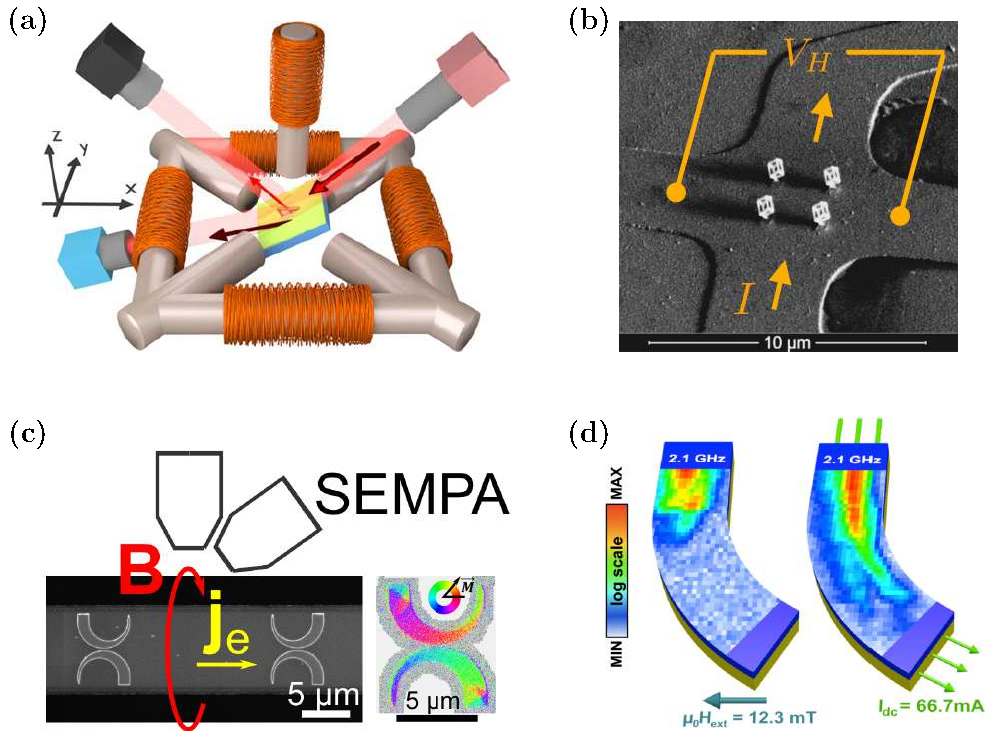
\includegraphics[width=0.85\textwidth]{fig_characterization_techniques}
	\caption{\label{fig:Characterization_techniques}%
		\textbf{Advanced characterization techniques for curvilinear nanomagnets.} \textbf{(a)}, Schematics of dark-field MOKE. Adapted with permission from~\cite{Sanz-Hernandez17}. \textbf{(b)}, Micro-Hall cross setup with nanocubes. Adapted with permission from~\cite{Mamoori18}. \textbf{(c)}, Sketch of SEMPA setup and color-coded image from flat curvilinear structures. Adapted with permission from~\cite{Schoenke20}. \textbf{(d)}, BLS intensity distribution of spin waves in a curved stripe. Adapted with permission from~\cite{Vogt12}.
	}
\end{figure}
%==================================================================/


\subsection{Magnetic characterization}

Magnetic characterization of flat curved magnetic geometries relies on different methods, that could be generalized in the following groups:
\begin{itemize}
	\item \textbf{Magnetometry techniques} utilize the stray field measurements to characterize magnetic responses from the particular geometrical structure. This could be an \textit{integral magnetometry techniques}, that provide the magnetic responses over the large-scale area and include the standard superconducting quantum interference device (SQUID) magnetometry, vibrating sample magnetometry (VSM) and magneto-optic Kerr effect (MOKE) magnetometry, that recently was improved for high-precision analysis of curvilinear structures by utilizing dark-field MOKE magnetometry~\cite{Sanz-Hernandez17}, see Fig.~\ref{fig:Characterization_techniques}(a). In addition to the integral methods, there are \textit{local magnetometry techniques} of the individual objects, which retrieve both the spatial distribution of the stray fields and magnetic properties. These methods includes dynamic cantilever-based~\cite{Degen09,Weber12,Mehlin18,Braakman19} and nano-SQUID magnetometries~\cite{Vasyukov18}.
	\item \textbf{Transport techniques} provide the insight into the charge and spin transport properties of magnetic objects. These techniques include the group of magneto-sensitive transport-based electrical measurements, that employs: anisotropic magnetoresistance (AMR), giant magnetoresistive (GMR), giant magnetoimpedance (GMI) effect, current-induced spin torques and Hall-magnetometry, see Fig.~\ref{fig:Characterization_techniques}(b).
	\item \textbf{Magneto-sensitive visualization techniques} provide a valuable information about the magnetization textures of curvilinear magnetic objects. These techniques include \textit{scanning-probe methods}, e.g. MFM, that provide a spatial resolution up to 50~nm for curved  nanoobjects~\cite{Albrecht12,Nguyen15,Streubel16,Ball17,May19}; electron-based methods, including Lorentz transmission electron microscopy (TEM)~\cite{Phatak11,Phatak12,Nord19} with its extension to electron holography, that allows to perform the detail static reconstruction of magnetic textures in flat curved geometries~\cite{Klaeui05,Nord19}; scanning electron technique with polarization analysis~(SEMPA)~\cite{Klaui05,Schoenke18,Schoenke20}, see Fig.~\ref{fig:Characterization_techniques}(c); X-ray-based visualization methods, including X-ray magnetic circular dichroism photoelectron emission microscopy (XMCD-PEEM)~\cite{Streubel15c,Streubel15,Streubel16,Volkov19,Volkov19c}.   
	\item \textbf{Dynamic magnetization methods} rely on time domain and provide input on evolution of magnetization textures and spin dynamics. These techniques include the ferromagnetic resonance (FMR) methods~\cite{Liedke13}, whose sensitivity for the study of curved magnetic objects could be substantially improved by utilizing microresanator loops~\cite{Lenz19}. Another valuable dynamic measurement method is Brillouin light spectroscopy (BLS)~\cite{Demokritov01}, that recently was improved by using high-sensitive BLS microscopy~\cite{Vogt12,Vogt14,Schultheiss19}, see Fig.~\ref{fig:Characterization_techniques}(d). Also, it should be mentioned the possibility to perform dynamic magnetic imaging using scanning transmission X-ray microscope (STXM)~\cite{Wintz11,Streubel15,Streubel15d,Wintz16,Woo16,Zimmermann18,Sluka19}.
\end{itemize}



%Magnetic characterization of flat curved structures utilizes the different methods, that could be generalized in the following groups:
%
%\subsection{Magnetometry techniques}
%
%This methods rely on measurements of magnetic responses from the curvilinear structures. Firstly, to this group should be included \textit{integral magnetometry} techniques, that provide the magnetic responses over the large-scale area and include the standard superconducting quantum interference device (SQUID) magnetometry, vibrating sample magnetometry (VSM) and magneto-optic Kerr effect (MOKE) magnetometry~\cite{Streubel12b,Streubel13c,Streubel14,Ueltzhoeffer16,Hunt20}, that recently was improved for high-precision analysis of curvilinear structures by utilizing dark-field MOKE magnetometry~\cite{Sanz-Hernandez17}, see Fig.~\ref{Fig:Experimental_figs_2}(a).
%
%In addition to the integral methods, there is a group of \textit{local magnetometry} techniques  of the individual object, that retrieve both the spatial distribution of the stray fields and magnetic properties. This group includes dynamic cantilever-based~\cite{Degen09,Weber12,Mehlin18,Braakman19} (Fig.~\ref{Fig:Experimental_figs_2}(b)) and nano-SQUID magnetometries~\cite{Vasyukov18} (Fig.~\ref{Fig:Experimental_figs_2}(c)). Here it should be referred the scanning reconfigurable magnetic force microscopy (MFM)~\cite{Kazakova19,May19,Corte-Leon19}, that allows to quantify the 3D magnetization pattern of a magnetic nanoobject from a 2D data~\cite{Vock14}, and micro-Hall magnetometry that was applied for magnetic characterization of complex-shapes FEBID nanostructures~\cite{Keller18,Mamoori18} (Fig.~\ref{Fig:Experimental_figs_2}(d)). 
%
%\begin{figure*}
%	\centering
%	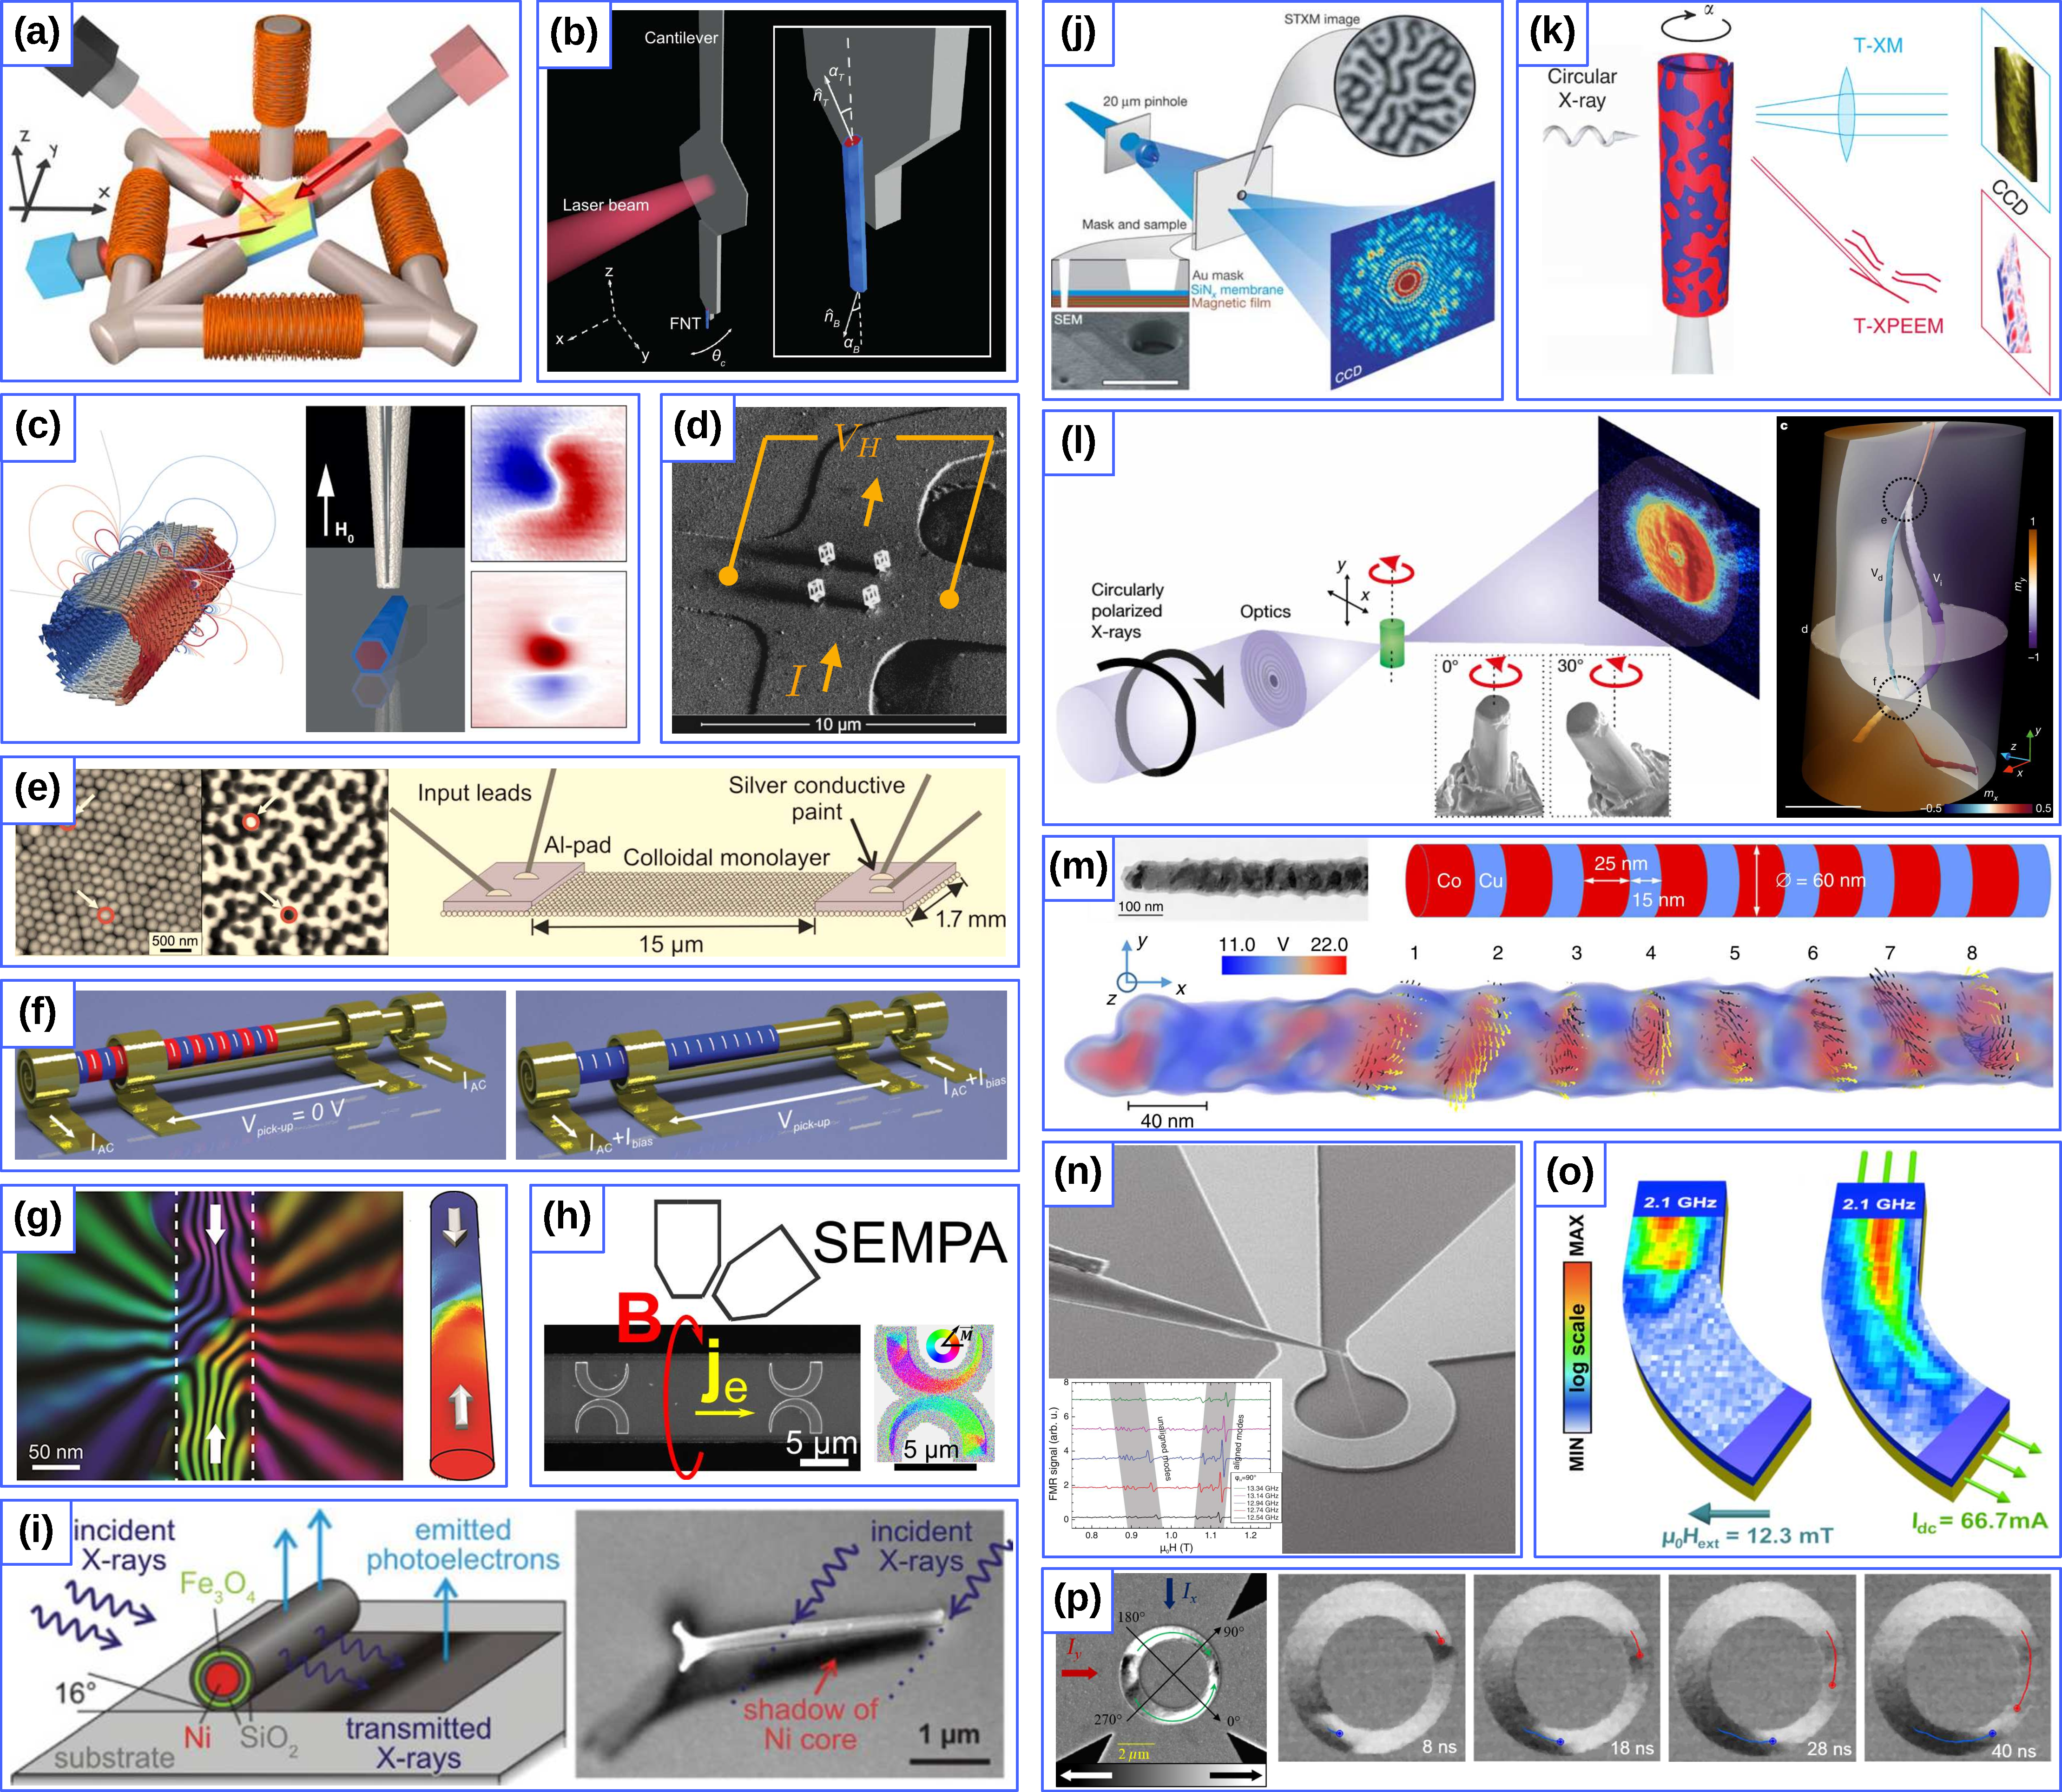
\includegraphics[width=0.97\linewidth]{fig_characterization.pdf}
%	\caption{\textbf{Advanced characterization techniques for curvilinear nanomagnets.} \textbf{(a)} Schematics of dark-field MOKE. Adapted with permission from~\cite{Sanz-Hernandez17}. \textbf{(b)} Dynamic cantiliver-based magnetometry tip with magnetic nanotube at the end. Adapted with permission from~\cite{Mehlin18}. \textbf{(c)} Nano-SQUID tip and reconstructed stray field of hexagonal magnetic nanotube. Adapted with permission from~\cite{Vasyukov18}. \textbf{(d)} Micro-Hall cross setup with nanocubes. Adapted with permission from~\cite{Mamoori18}. \textbf{(e)} Sketch of AMR measurements on self-assembled magnetic nanoparticles. Adapted with permission from~\cite{KimlingnMoser10}. \textbf{(f)} Schematics of an integrated GMI sensor operation. Adapted with the permission from~\cite{Karnaushenko15a}. \textbf{(g)} Electron holography of a DW in Ni nanocylinder. Adapted with permission from~\cite{Biziere13}. \textbf{(h)} Sketch of SEMPA setup and color-coded image from flat curvilinear structures. Adapted with permission from~\cite{Schoenke20}. \textbf{(i)} XMCD-PEEM technique for 3D magnets with shadow contrast reconstruction. Adapted with permission from~\cite{Kimling11}. \textbf{(j)} (i) X-ray spectro-holography. Adapted with permission from~\cite{Eisebitt04}.
%		\textbf{(k)} Concept of MXT based on a combination of STXM and XMCD-PEEM techniques for the 3D magnets. Adapted with permission from~\cite{Streubel15a}. \textbf{(l)} Hard X-Ray magnetic tomography setup based on ptychographic scans of a sample. Adapted with permission from~\cite{Donnelly17}.	\textbf{(m)} Holographic vector field electron tomography of 3D nanomagnets. Adapted with permission from~\cite{Wolf19}. \textbf{(n)} FMR measurements of a magnetic nanowire in $\Omega$-shaped resonator. Adapted with permission from~\cite{Lenz19}. \textbf{(o)} BLS intensity distribution of spin waves in a curved stripe. Adapted with permission from~\cite{Vogt12}. \textbf{(p)} Asymmetric ferromagnetic ring and STXM snapshots of automotive DWs motion. Adapted with permission from~\cite{Mawass17}.} 
%	\label{Fig:Experimental_figs_2}
%\end{figure*}

%\subsection{Transport techniques}
%
%This group of techniques provide the insight into the charge and spin transport properties of magnetic materials. These techniques include the group of magneto-sensitive transport-based electrical measurements, that employs: anisotropic magnetoresistance (AMR) effect for nanotubes~\cite{Rueffer12,Zimmermann18}, monolayer of magnetic spherical caps~\cite{KimlingnMoser10} (Fig.~\ref{Fig:Experimental_figs_2}(e)), ferromagnetic microhelices~\cite{Maurenbrecher18} and nanomembranes~\cite{Moench11,Schumann12,Muller12}; giant magnetoresistive (GMR) effect for nanomembranes~\cite{Mueller12}; giant magnetoimpedance (GMI) effect~\cite{Karnaushenko15a} Fig.~\ref{Fig:Experimental_figs_2}(f); current-induced spin torques~\cite{Schoebitz19}. 

%\subsection{Magneto-sensitive visualization techniques}
%
%A valuable information about the magnetization textures of curvilinear objects can be obtained by magneto-sensitive visualization techniques, that provide access to complex magnetization patterns on curved magnetic systems. These techniques include \textit{scanning-probe methods}, e.g. MFM, that provide a spatial resolution up to 50~nm for curved nanoobjects~\cite{Ulbrich06,Makarov07,Makarov08,Makarov09,Schulze10,Albrecht12,Nguyen15,Streubel16,Ball17,May19}; MOKE microscopy~\cite{Streubel12b,Streubel13c,Streubel14,Ueltzhoeffer16,Hunt20}, that recently was enabled for pump-probe time-resolved measurements of micro-tetrapod geometries~\cite{Sahoo18}; electron-based methods, including Lorentz transmission electron microscopy (TEM)~\cite{Phatak12,Phatak11} with its extension to electron holography, that allows to perform the detail static reconstruction of magnetic textures in flat~\cite{Klaeui05,Nord19} and 3D~\cite{Biziere13,Phatak14,Phatak20} curved geometries, see Fig.~\ref{Fig:Experimental_figs_2}(g); scanning electron technique with polarization analysis~(SEMPA)~\cite{Schoenke18}, that is suitable for imaging flat curved magnetic geometries~\cite{Klaui05,Schoenke20}, see Fig.~\ref{Fig:Experimental_figs_2}(h); X-ray-based visualization methods, including X-ray magnetic circular dichroism photoelectron emission microscopy (XMCD-PEEM)~\cite{Streubel15c,Streubel15,Streubel16,Volkov19,Volkov19c}.  
%
%While these methods are limited to the analysis of simple magnetic geometries, the visualization of complex 3D shape geometries requires the utilization of the tomographic-based approaches. Thus, MOKE microscopy~\cite{Streubel14}, that recently was enabled for tomography-like screening of bulk samples~\cite{Schaefer20}; XMCD-PEEM was successfully extended to image interior magnetization textures of complex curved magnetic nanoobjects by using transmission shadow contrasts~\cite{Kimling11,Streubel12,Streubel12b,Streubel14a,DaCol14,Stano18a,Wartelle18,Schoebitz19,Wartelle19}, see Fig.~\ref{Fig:Experimental_figs_2}(i). X-ray spectro-holography~\cite{Eisebitt04} could be also utilizes for the characterization of 3D curved magnetic nanostructures (Fig.~\ref{Fig:Experimental_figs_2}(j)), e.g. magnetically capped nanospheres~\cite{Guenther10}. Full field X-ray microscopy, that combines magnetic transmission
%soft X-ray microscopy (MXTM) with XMCD-PEEM, was successfully applied to realize the concept of soft X-ray magnetic tomography (MXT)~\cite{Streubel15a}, see Fig.~\ref{Fig:Experimental_figs_2}(k). Complementary, hard X-ray magnetic tomography with ptychographic scans potentially allows for 10 nm resolution of 3D magnetic textures~\cite{Donnelly17}, see Fig.~\ref{Fig:Experimental_figs_2}(l). The electron holography is extended to holographic vector field electron tomography~\cite{Wolf13,Wolf19}, see Fig.~\ref{Fig:Experimental_figs_2}(m), that allows to reconstruct 3D magnetic textures with a sub 10~nm resolution. 

%\subsection{Dynamic magnetization methods}
%
%Other methods, that rely on time domain and provide input on magnetization characterization are dynamic methods. These techniques include the ferromagnetic resonance (FMR) methods~\cite{Liedke13}, whose sensitivity for the study of curved magnetic objects could be substantially improved by utilizing microresanator loops~\cite{Lenz19}, see Fig.~\ref{Fig:Experimental_figs_2}(n). Another valuable dynamic measurement method is Brillouin light spectroscopy (BLS)~\cite{Demokritov01}, that recently was improved by using high-sensitive BLS microscopy~\cite{Vogt12,Vogt14,Schultheiss19}, see Fig.~\ref{Fig:Experimental_figs_2}(o). Also, it should be mentioned the possibility to perform dynamic magnetic imaging using scanning transmission X-ray microscope (STXM)~\cite{Wintz11,Streubel15,Streubel15d,Wintz16,Woo16,Zimmermann18,Sluka19}, see Fig.~\ref{Fig:Experimental_figs_2}(p).



%These techniques include the scanning-probe near-field methods, that are represented by: scanning reconfigurable magnetic force microscopy (MFM)~\cite{Kazakova19,May19,Corte-Leon19}, nano-superconducting quantum interference device magnetometry~\cite{Vasyukov18} and dynamic cantilever magnetometries~\cite{Degen09,Weber12,Mehlin18,Braakman19}. These methods allow to retrieve the magnetic properties and magnetization configuration from the demagnetizing fields of curvilinear structures. To the magnetometry techniques should be also included the group of magneto-sensitive transport-based electrical measurements, that employs: anisotropic magnetoresistance (AMR) effect for nanotubes~\cite{Rueffer12,Zimmermann18}, monolayer of magnetic spherical caps~\cite{KimlingnMoser10}, ferromagnetic microhelices~\cite{Maurenbrecher18} and nanomembranes~\cite{Moench11,Schumann12,Muller12}; giant magnetoresistive (GMR) effect for nanomembranes~\cite{Mueller12}; giant magnetoimpedance (GMI) effect~\cite{Karnaushenko15a}; micro-Hall magnetometry that was applied for magnetic characterization of complex-shapes FEBID nanostructures~\cite{Keller18,Mamoori18}; current-induced spin torques~\cite{Schoebitz19} and spin-orbit torques~~\cite{Miron10,Miron11a,Garello13,Manchon19}; magneto-optic Kerr effect (MOKE) magnetometry~\cite{Streubel12b,Streubel13c,Streubel14,Ueltzhoeffer16,Hunt20}, that recently was improved for high-precision analysis of curvilinear structures by utilizing dark-field MOKE magnetometry~\cite{Sanz-Hernandez17}.




% To these techniques should be also referred the mentioned above \textit{scanning-probe methods}, including MFM, that provide a spatial resolution up to 50~nm for curved nanoobjects~\cite{Ulbrich06,Makarov07,Makarov08,Makarov09,Schulze10,Albrecht12,Nguyen15,Streubel16,Ball17,May19}. MOKE microscopy~\cite{Streubel14}, that recently was enabled for tomography-like screening of bulk samples~\cite{Schaefer20} and pump-probe time-resolved measurements of micro-tetrapod geometries~\cite{Sahoo18}. The high-resolution magnetic imaging of curved geometries is achieved by means of different X-ray-based visualization methods, including X-ray magnetic circular dichroism photoelectron emission microscopy (XMCD-PEEM)~\cite{Streubel15c,Streubel15,Streubel16,Volkov19,Volkov19c}, that was successfully extended to image interior magnetization textures of complex curved magnetic nanoobjects by using transmission shadow contrasts~\cite{Kimling11,Streubel12,Streubel12b,Streubel14a,Wartelle18,Schoebitz19,Wartelle19}, see Fig.~\ref{Fig:Experimental_figs_2}(b), and subsequently modified to the concept of soft X-ray magnetic tomography (MXT)~\cite{Streubel15a}, see Fig.~\ref{Fig:Experimental_figs_2}(c), and hard X-ray magnetic tomography with ptychographic scans potentially allows for 10 nm resolution of 3D magnetic textures~\cite{Donnelly17}, see Fig.~\ref{Fig:Experimental_figs_2}(a). It should be mentioned also the possibility to utilize the X-ray spectro-holography~\cite{Eisebitt04} for the characterization of microscopic magnetically capped nanospheres~\cite{Guenther10}. Another valuable imaging techniques are electron-based methods, including scanning electron technique with polarization analysis~(SEMPA)~\cite{Schoenke18}, that is suitable for imaging flat curved magnetic geometries~\cite{Klaui05,Schoenke20}, Lorentz transmission electron microscopy (TEM)~\cite{Phatak12,Phatak11} with its extension to electron holography, that allows to perform the detail static reconstruction of magnetic textures in flat~\cite{Klaeui05,Nord19} and 3D~\cite{Phatak14,Phatak20} curved geometries, and its further extension to holographic vector field electron tomography~\cite{Wolf13,Wolf19}, see Fig.~\ref{Fig:Experimental_figs_2}(d), that allows to reconstruct 3D magnetic textures with a sub 10~nm resolution.


%The \textbf{characterization of magnetic responses} from 3D curvilinear objects utilizes (I) a high-resolution magneto-sensitive visualization techniques, that enable a direct reconstruction of the magnetization distribution in 3D object,  and (II) advanced magnetometry techniques, that indirectly infer the magnetic configuration of nanosctructure, as demonstrated in Fig.~\ref{Fig:Experimental_figs_2}. The first type of techniques is based on the high-resolution vector tomography, e.g. the hard X-Ray magnetic tomography with ptychographic scans potentially allows for 10 nm resolution of 3D magnetic textures~\cite{Donnelly17}, see Fig.~\ref{Fig:Experimental_figs_2}(a). Soft X-Ray magnetic circular dichroism photoelectron emission microscopy (XMCD-PEEM) was successfully applied to image interior domain patterns in nanorods relying on a transmission shadow contrast~\cite{Kimling11}, see Fig.~\ref{Fig:Experimental_figs_2}(b). This method was modified to the concept of soft X-ray magnetic tomography (MXT)~\cite{Streubel15a}, see Fig.~\ref{Fig:Experimental_figs_2}(c). Another valuable tomographic method, that allows to reconstruct magnetic textures with a sub 10 nm resolution, is holographic vector field electron tomography~\cite{Wolf13,Wolf19}, see Fig.~\ref{Fig:Experimental_figs_2}(d). It should be mentioned also the possibility to utilize the X-ray spectro-holography~\cite{Eisebitt04} for the characterization of microscopic magnetically capped nanospheres~\cite{Guenther10}. 

%The second type of experimental methods relies on the novel magnetometry techniques, that rely on the indirect measurements of magnetic responses from the curvilinear structures. There are optical, electrical and near-field high-sensitive magnetometry methods. The first type of magnetometry techniques is based on the magnetooptical Kerr effect (MOKE) and Brillouin light spectroscopy (BLS)~\cite{Demokritov01} methods. Recently, the standard MOKE was developed for high-precision analysis of curvilinear structures by utilizing dark-field MOKE magnetometry~\cite{Sanz-Hernandez17}, pump-probe time-resolved MOKE measurements~\cite{Sahoo18}  and tomography-like MOKE screening of bulk samples~\cite{Schaefer20}, while the convenient BLS method was improved by using high-sensitive BLS microscopy~\cite{Vogt12,Vogt14,Schultheiss19}. The group of electrical magnetometry techniques is based on the resistance measurements of magnetic samples in external field, that employs magnetoresistance~\cite{KimlingnMoser10,Maurenbrecher18}, micro-Hall~\cite{Keller18,Mamoori18} effects and current-induced spin-orbit torques in magnetic systems~\cite{Miron10,Miron11a,Garello13,Manchon19}. The near-field magnetometry method are represented by a scanning reconfigurable magnetic force microscopy (MFM)~\cite{Kazakova19,May19,Corte-Leon19}, nano-superconducting quantum interference devices~\cite{Vasyukov18} and dynamic cantilever magnetometries~\cite{Mehlin18}. 
